\documentclass[pre,twocolumn,superscriptaddress,showpacs]{revtex4-2}

\usepackage[utf8]{inputenc}
\usepackage{amsmath,amssymb}
\usepackage{bm}
\usepackage{graphicx}
\usepackage{dcolumn}
\usepackage{booktabs}
\usepackage{xcolor}
\usepackage[colorlinks=true,linkcolor=blue,citecolor=blue,urlcolor=blue]{hyperref}

\graphicspath{{figs/}}
\providecommand{\todo}[1]{{\color{red}\textbf{[TODO}\ifx\relax#1\relax\else: #1\fi\textbf{]}}}
\newcommand{\repourl}{\url{https://github.com/jfbonder/universe25-abm}}
\newcommand{\zenododoi}[1]{\href{https://doi.org/#1}{doi:#1}}
\newcommand{\extended}{the extended version in the repository}

\begin{document}

\title{An Agent-Based Model for the Social Collapse of Calhoun's Universe~25 Experiment}

\author{Julián Fernández Bonder}
\email{jfbonder@dm.uba.ar}
\affiliation{Departamento de Matemática, FCEN, Universidad de Buenos Aires, Buenos Aires, Argentina}
\affiliation{Instituto de Cálculo, UBA--CONICET, Buenos Aires, Argentina}

\date{\today}

\begin{abstract}
We ask which \emph{local} interaction rules suffice to reproduce, qualitatively, the social collapse of Calhoun's
Universe~25, where a mouse colony with unlimited resources stopped reproducing and died out.
In a lattice agent-based model each individual carries a partly inherited social state that deteriorates under
crowding; seventeen observed patterns are evaluated run by run against null models.
Crowding and a long-lived demography alone produce the envelope of the collapse: a peak well below
capacity, the end of natality, largely the social failure of late-born cohorts, and extinction.
Four local rules (a juvenile plasticity window, social learning, crowd aversion and refuges of limited capacity) add
coexisting crowded and isolated deteriorated classes, absent from most null models; the persistence of the isolated
class follows from the refuge design.
The full set of patterns holds in 99.5\% of the runs; with a small background mortality or spread initial ages it
falls to 55--63\%, only through a generic timing criterion.
The dynamics is a boom of one or two generations, not Calhoun's multi-generational sequence.
\end{abstract}

\maketitle

\section{Introduction}
\label{sec:intro}

Beginning in July 1968, John B.~Calhoun followed a population of house mice in a closed enclosure that he called
\emph{Universe~25}, in which food, water and nest space were in excess, predators and epidemic disease were
excluded, and emigration was impossible \cite{Calhoun1973}. From four founding pairs the colony grew roughly
exponentially and stopped growing at about 2200 animals, well below the 3840 that the nest boxes could shelter. The
last young to survive weaning were born shortly after the peak, and the population then aged out without ever
recovering. Along the way Calhoun described a breakdown of social behaviour: withdrawn males gathered in pools at
the centre of the floor, nursing females attacked and abandoned their young, and there appeared the unwounded,
non-reproducing ``beautiful ones.'' Small groups moved to uncrowded enclosures during the decline did not reproduce,
even with partners raised without crowding (Marsden's work, reported in Ref.~\cite{Calhoun1973}; see also
Ref.~\cite{Marsden1972}). Calhoun read the collapse as a failure of social roles, not of resources: ``density per se was not the major factor'' \cite{Calhoun1973}.

The interpretation of the experiment has always been contested. Its popular message, ``density causes pathology,''
departed from Calhoun's own emphasis on social roles and design \cite{RamsdenAdams2009,Ramsden2009,AdamsRamsden2024},
and studies of human crowding found weak or no effects of density per se \cite{Galle1972,Freedman1975}. In earlier
confined rodent populations with abundant food, growth stopped through reduced litter survival mediated by social
interference \cite{Southwick1955,Lidicker1965}, and the maternal transmission of individual quality produces
delayed density dependence in models of population cycles \cite{GinzburgTaneyhill1994,InchaustiGinzburg1998}. For modelling, the decisive limitation is
that Universe~25 was a single realization; Calhoun himself called the study ``observation and reconstruction of a
process; it was historical'' \cite{Calhoun1973}. A model tuned to the published curve therefore risks fitting one
sample path of a strongly stochastic process \cite{GwizdallaDus2026}. The recent agent-based simulation of
Gwizdałła and Duś \cite{GwizdallaDus2026} calibrates the growth phase against
the reported counts and produces the decline through deviation factors that switch on when the \emph{total}
population exceeds critical values; other accounts invoke the loss of uncertainty about the social hierarchy in a
game-theoretic setting \cite{Mantzaris2025} or fit maximum-entropy unimodal curves without a mechanistic model
\cite{Roman2025}.

We ask instead which \emph{local} interaction rules, with unlimited resources and no rule that depends on the total
population, generate robustly across stochastic realizations the part of Calhoun's sequence that runs from rapid
growth to extinction: deceleration with social deterioration, cessation of reproduction near the peak, a decline
without recovery, and differentiated classes of deteriorated animals. The latency phase and the growth from four
founding pairs are part of that sequence, but we do not claim them (Sec.~\ref{sec:discussion}).

Our core model is a lattice model in which each mouse carries an age, a sex and a continuous social state
$s_i\in[0,1]$. The social state deteriorates under local crowding, scales conception and pup survival, and is partly
inherited; movement is biased towards acquaintances. We add four local rules, each with a neutral value that
switches it off and recovers the core model, and each motivated by an observation of the original report (Sec.~\ref{sec:model}): a
juvenile window of social plasticity (R1), social learning of competence (R2), crowd aversion of deteriorated
animals (AV), and refuges of limited capacity preferred by deteriorated animals (R7). Following pattern-oriented
modelling \cite{Grimm2005}, we translate Calhoun's report into seventeen falsifiable patterns, each with an
operational criterion evaluated run by run, and we measure the discriminating power of every essential criterion
against four null models: no crowding damage; full inheritance without social learning; the long-lived demography
without the new rules; and the calibrated candidate without its four rules (Sec.~\ref{sec:methods}). Seven
hypotheses were preregistered before the production runs, and every deviation from that plan is reported.

Our main result is negative, and it is controlled by the null models: \emph{the envelope is generic; the rules add
the classes}. Crowding damage and a long-lived demography alone already produce the envelope of the collapse---a
peak well below capacity with free space, the end of natality near the maximum, the social failure of late-born
cohorts when they are scored at the end of the plasticity window, and extinction. These patterns verify that the
model has a boom and its end; they are not evidence for the rules. What the rules add, and most null models lack,
is the coexistence of crowded and isolated deteriorated classes. The persistence of the isolated class follows from
the refuge design, and the failure of transplanted late-phase animals to found a colony from the plasticity window;
we report both as consistency checks, not findings. Second, the simulated dynamics is a boom of one or two generations, not Calhoun's
multi-generational cascade: about 70\% of the births are to the founding animals, and the net reproductive number
falls from 3.8 to 0.4 in a single generation. Third, the full set of patterns holds in 99.5\% of the runs of the
reference candidate, but this overstates its robustness: with a small background mortality or with spread initial
ages it falls to 55--63\%, only through a generic criterion on the timing of the end of natality, while the patterns
that the rules add pass in every run (Sec.~\ref{sec:results}). The minimal set of rules (R1, R2 and R7) is minimal
only at the evaluation thresholds used.

The ODD description, the full tables of patterns and null models, and the robustness analyses are given in the
Supplemental Material; the calibration, the mean-field analysis and the remaining results are in an extended version, available with the full ODD description, the code and the data in the repository \repourl.

\section{Model}
\label{sec:model}

The model is an individual-based, discrete-time stochastic process on a lattice, with one step per week. Each
individual has a position, an age, a sex, a sparse affinity memory and a \emph{social state} $s_i\in[0,1]$, its
capacity for normal social and reproductive behavior. All rules are local: no individual knows the population size. The \emph{core model}
(lattice, affinity, movement with attraction, crowding damage, reproduction and senescent mortality) is extended by
four rules, R1, R2, AV and R7, each with a neutral value that switches it off and recovers the core model
(Fig.~\ref{fig:model-schematic}, Table~\ref{tab:params}; ODD in the Supplemental Material).

\begin{figure}[t]
  \centering
  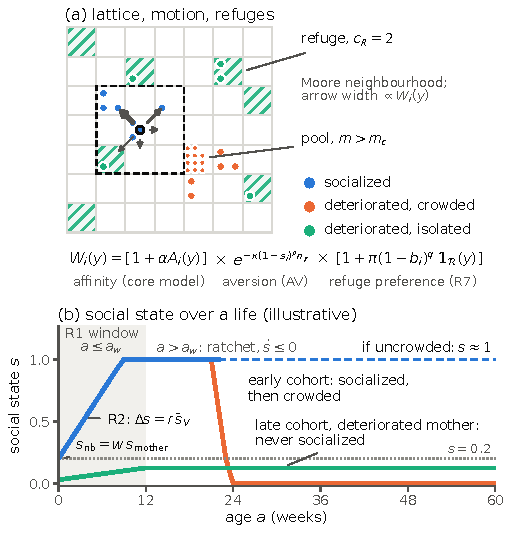
\includegraphics[width=\columnwidth]{model_schematic_pre.pdf}
  \caption{Schematic of the model.
  (a)~A focal agent (ringed) chooses a cell of its Moore neighborhood (dashed) with the weight of
  Eq.~\eqref{eq:model-move}, whose three factors are shown below the lattice; arrow width is proportional to the
  weight. Deteriorated individuals gather in pools ($m>m_c$) or occupy refuges (hatched, capacity $c_R=2$).
  (b)~Illustrative trajectories of $s$ versus age, from Eqs.~\eqref{eq:model-social} and~\eqref{eq:model-learning}
  with fixed environments (not a simulation). A pup starts at $w\,s_{\rm mother}$ and gains competence only inside
  the window $a\le a_w$ (R1), at a rate set by its neighbors (R2); afterwards crowding can only lower $s$.}
  \label{fig:model-schematic}
\end{figure}

\subsection{Core model}
\label{sec:model-baseline}

\paragraph*{Space, affinity and movement.}
Individuals live on an $L\times L$ lattice $G$ ($L=30$, $|G|=900$) with hard walls and no occupancy limit; $m_i$ is
the occupancy of the cell of $i$, itself included. Pairs at Chebyshev distance $\le1$ reinforce their affinity,
$F_{ij}\leftarrow(1-\eta)F_{ij}+\eta$, and the others decay, $F_{ij}\leftarrow(1-\delta)F_{ij}$: the memory,
$1/\delta=100$ weeks, is long and built only by proximity. Every week all individuals move simultaneously to one of
the nine cells $y$ of their Moore neighborhood, own cell included, with probability proportional to
\begin{equation}
  \begin{split}
  W_i(y)={}&\bigl[1+\alpha A_i(y)\bigr]\,e^{-\kappa(1-s_i)^{p}n_y}\\
           &\times\bigl[1+\pi(1-b_i)^{q}\,\mathbf 1_{\mathcal R}(y)\bigr],
  \end{split}
  \label{eq:model-move}
\end{equation}
where $A_i(y)=\sum_{j\in y}F_{ij}$, $n_y$ is the number of \emph{other} individuals in $y$, $\mathcal R$ is the set
of non-full refuges (refuge cells with $n_y<c_R$), and $\mathbf 1_{\mathcal R}(y)=1$ if $y$ is a non-full refuge and 0
otherwise; full refuges cannot be entered (R7, below). The core model has only the first factor, the attraction $\alpha$ towards acquaintances; the
other two are the rules AV and R7.

\paragraph*{Social state.}
After moving,
\begin{equation}
  s_i\leftarrow\min\bigl\{1,\max\bigl[0,\;s_i+\varrho_i-\gamma\,(m_i-m_c)_+\bigr]\bigr\},
  \label{eq:model-social}
\end{equation}
where $\gamma(m_i-m_c)_+$ is the damage inflicted by each occupant in excess of the community size $m_c$, and in the
core model recovery is a constant, $\varrho_i=r$. Deterioration is local, density-triggered and, being convex in the
occupancy, acts as a switch.

\paragraph*{Demography.}
A reproductive female ($a_{\min}\le a\le a_{\rm rep}$) sharing her cell with a reproductive male conceives with
probability $p_{\rm conc}=p_0\,s_f\,s_m$; each pup of the litter (mean 6.55) survives birth with probability $q_0\,s_f$
and is born with $s_{\rm nb}=w\,s_f+(1-w)\,s_0$ (full inheritance, $w=1$, in the core model). Death is senescent, with
weekly probability $\{1+\exp[-k(a-a_{\max})]\}^{-1}$, independent of $s$ (an optional social advance of
senescence, $\mu_s$, is zero in every model): the beautiful ones were ``physically
healthy''~\cite{Calhoun1973}, so the absence of social deaths (A4) and the senescent decline (O8) hold by
construction. The long-lived demography of the candidates ($a_{\max}=120$, $a_{\rm rep}=80$ weeks) matches the menopause at about 560
days and the longevity of about 800 days in Universe~25~\cite{Calhoun1973}. With no mortality before senescence the
population sits on a plateau once natality stops. Initially $200+200$ individuals of age 4 weeks with $s=1$ are placed at random.

\paragraph*{Controls.}
A rule is switched off by its neutral value: $a_w=\infty$ (R1); $\lambda=0$ with $w=1$ and individual recovery at
$r=0.01$ (R2); $\kappa=0$ (AV); no refuges (R7). The \emph{short-lived control} is the core model with all four rules
switched off, attraction $\alpha=1.4$ and a short life span, $a_{\max}=60$ and $a_{\rm rep}=50$ weeks; the
\emph{long-lived control} is the same with $a_{\max}=120$ and $a_{\rm rep}=80$ (Table~\ref{tab:params}). The null
models are defined relative to \textsf{C1} in Sec.~\ref{sec:methods}.

\subsection{Minimal additional rules}
\label{sec:model-rules}

With the long-lived demography and $\alpha=4$, crowding alone already produces the envelope of the collapse, but not
coexisting classes of deteriorated animals (Sec.~\ref{sec:results}). Each rule is motivated by an observation of the
original report~\cite{Calhoun1973}; R7 (five parameters and a hard capacity) was designed after a candidate without
refuges had failed to produce a persistent isolated class.

\paragraph*{R1: juvenile plasticity window ($a_w$).}
Recovery is possible only for $a\le a_w=12$ weeks ($\varrho_i=0$ otherwise), while crowding damage acts at every age: an adult
is a ratchet, $\dot s_i\le0$, and recovery becomes a lineage process. Since $p_{\rm conc}\propto s_fs_m$, an adult with
$s\simeq0$ can neither recover nor reproduce, whatever its partner. \emph{Motivation:} mice moved in mid-phase~D to
uncrowded universes, even with partners matured without crowding, never recovered reproductive behavior (Marsden's
work~\cite{Calhoun1973,Marsden1972}); the failure of phase-D transplants (O12) is thus a
consistency check of R1. \emph{Mechanism:} refuges are pockets of low density in which, without R1, deteriorated
animals recover and breed again (natality resumes and the primary outcome falls to 0.21), whereas without refuges the
collapse stays irreversible in most runs even without R1 (O6 and O7 in 0.85 of 40 runs). R1 is what lets a persistent isolated class
coexist with an irreversible collapse.

\paragraph*{R2: social learning ($\lambda$, with partial inheritance $w$).}
Recovery is \emph{learned} from the neighbors,
\begin{equation}
  \varrho_i=r\bigl[(1-\lambda)+\lambda\,\bar s_{V(i)}\bigr],
  \label{eq:model-learning}
\end{equation}
with $\bar s_{V(i)}$ the mean state of the other individuals of the $3\times3$ block centred on $i$ (0 if none).
With R1 it acts only on juveniles, which start with a fifth of their mother's competence ($w=0.2$, $s_0=0$) and can
gain at most $r\,a_w=1.2$ from competent neighbors. For $\lambda=1$, $s=0$ is absorbing for the population, not only
for the individual: without competent adults pups have nobody to learn from.
\emph{Motivation:} ``by midway in phase~C essentially all young were prematurely rejected by their
mothers''~\cite{Calhoun1973}. Pups are born at $s_{\rm nb}\le0.2$, the patterns' threshold for ``deteriorated,'' so
part of the failure of crowded-born cohorts is definitional (Sec.~\ref{sec:results}); the essential part of R2 is
learning, not inheritance ($w=0$ with $r=0.15$ passes in all 120 runs).

\paragraph*{AV: crowd aversion of the deteriorated ($\kappa$).}
The factor $e^{-\kappa(1-s_i)^{p}n_y}$ of Eq.~\eqref{eq:model-move}, with $p=4$, acts only for $s\lesssim0.3$.
Facing a cell of $n$ acquaintances ($A\simeq n$), a deteriorated individual maximizes $(1+\alpha n)e^{-\kappa n}$ at
$n^*=1/\kappa-1/\alpha\approx6.4\approx0.8\,m_c$ and avoids cells of strangers, so the deteriorated split between
pools, where damage continues, and nearly empty cells. \emph{Motivation:} withdrawn males pooled and wounded each other; the beautiful ones ``never engaged in
fighting''~\cite{Calhoun1973}. Without refuges AV alone generates the isolated class; with refuges it is not needed for
the primary outcome and instead shapes the use of space, \emph{reducing} the empty fraction of cells at the peak
(Sec.~\ref{sec:results}).

\paragraph*{R7: refuges of hard capacity ($\pi$).}
A fixed random fraction $f_R$ of the cells are refuges that hold at most $c_R=2$ individuals (a hard capacity:
residents keep their place, rejected entrants return). The deteriorated prefer refuges through the factor $1+\pi(1-b_i)^{q}$ of Eq.~\eqref{eq:model-move}, with $b_i=s_i$. The total capacity,
$f_Rc_R|G|=540$ places or about 20\% of the adults at the peak, bounds the persistently isolated fraction. The hard
capacity remedies the stampedes of synchronous moves (Sec.~\ref{sec:results}). \emph{Motivation:} withdrawn females retreated to the high, less preferred nest
boxes~\cite{Calhoun1973}, the analogue of the refuges if a cell is a nest box; but $c_R=2$ is the isolation threshold
$m\le2$ of O13, a design choice that makes the persistence of the isolated class (O13p) hold by construction.

\paragraph*{Candidates and time scales.}
\label{sec:model-candidates}
Rules and parameters were chosen to maximize the number of patterns reproduced with the fewest rules, not by fitting a curve,
and with the evaluator later used to report them, so calibration is not validation (Sec.~\ref{sec:methods}). The reference candidate \textsf{C1} has the four rules. \textsf{C1$'$} omits AV
and is the minimal set for the preregistered primary outcome O17p (each single ablation gives O17p $=0$ in 40 runs),
but only at the evaluation thresholds: it passes in 0.835 [0.78, 0.88] of the runs, against 0.995 for \textsf{C1}.
Deterioration takes about one
generation: the animals past the window lose half of their competence $t_{\rm det}\approx10$ weeks after crowding sets
in, and $\Gamma=t_{\rm det}/T_{\rm gen}\approx1.1$ (0.7 with the mean age of the mothers at birth as $T_{\rm gen}$), a
heuristic of scales against $\Gamma\approx3.5$ for Universe~25 (our estimate, with a different operational
definition) that does not set the depth of the boom.

\begin{table}[t]
  \caption{Parameters of the reference candidate \textsf{C1} and of the short-lived control (SL); \textsf{C1$'$}
  is \textsf{C1} with $\kappa=0$, and the long-lived control is SL with $a_{\max}=120$ and $a_{\rm rep}=80$. Time in weeks; a dash means that the rule is inactive. The $N_0$ initial individuals
  have age 4 weeks and $s=1$. Presets \texttt{calhoun\_C1} and \texttt{calhoun\_C1p} of the \texttt{u25} package.}
  \label{tab:params}
  \begin{ruledtabular}
  \begin{tabular}{lcclcc}
    Symbol & \textsf{C1} & SL & Symbol & \textsf{C1} & SL \\
    \hline
    $L$ & 30 & 30 & $a_w$ (R1) & 12 & $\infty$ \\
    $N_0$ & 400 & 400 & $\lambda$ (R2) & 1 & 0 \\
    $\alpha$ & 4 & 1.4 & $w,\ s_0$ (R2) & 0.2, 0 & 1, -- \\
    $\eta,\ \delta$ & 0.2, 0.01 & 0.2, 0.01 & $\kappa,\ p$ (AV) & 0.15, 4 & -- \\
    $m_c,\ \gamma$ & 8, 0.1 & 8, 0.1 & $f_R,\ c_R$ (R7) & 0.3, 2 & -- \\
    $r$ & 0.1 & 0.01 & $\pi,\ q,\ b_i$ (R7) & 100, 4, $s_i$ & -- \\
    $p_0,\ q_0$ & 0.3, 0.95 & 0.3, 0.95 & $a_{\min},\ a_{\rm rep}$ & 6, 80 & 6, 50 \\
    $\mu_s$ & 0 & 0 & $a_{\max},\ k$ & 120, 0.15 & 60, 0.15 \\
  \end{tabular}
  \end{ruledtabular}
\end{table}

\providecommand{\extended}{the extended version in the repository}
\section{Patterns, null models and statistical design}
\label{sec:methods}

\paragraph{Patterns.}
Universe~25 is a single realization, so we do not fit its population curve. We extract from Calhoun's report
\cite{Calhoun1973} seventeen qualitative, falsifiable patterns (O1--O17) and four anti-patterns (A1--A4), each
translated into an operational criterion on simulated time series, and evaluate every criterion as a
\emph{distribution over stochastic replicates}, in the spirit of pattern-oriented modelling \cite{Grimm2005}. A
criterion returns PASS, MARGINAL, FAIL or NOT APPLICABLE (NA) for each run; for an ensemble we report the fraction
$f$ of PASS runs with a 95\% Wilson interval. An essential (E) pattern is reproduced if $f\ge0.8$, a desirable (D)
pattern if $f\ge0.5$. One model step is one week, and Calhoun's dates enter only through dimensionless ratios of
the peak time $t_{\rm pk}$, the peak size $N_{\rm pk}$ and the end of surviving births $t_{B0}$.
Table~\ref{tab:observations} summarizes the patterns; the full operational definitions and the numbers taken from
the report are in the Supplemental Material (SM), Tables~S1 and~S2. Patterns that follow from the rules by
construction are marked $^\ddagger$ and reported as consistency checks, not as findings: O12 from R1 together with
$p_{\rm conc}\propto s_fs_m$, O13p from R7 with $c_R=2$, and O8 and A4 from the absence of social mortality
(Sec.~\ref{sec:model}).

\begin{table*}[t]
\centering
\caption{Qualitative patterns (O) and anti-patterns (A) of Universe~25 \cite{Calhoun1973}, with their operational
criteria in short form (full definitions in the SM, Table~S1). E = essential, D = desirable, X = exploratory.
$^\S$Not preregistered: the preregistered form also passes in null models (SM, Table~S5).
$^\ddagger$Holds by construction (consistency check). $^\dagger$Not preregistered (defined after calibration).
$t_{\rm pk}$, $N_{\rm pk}$: time and size of the peak; $t_{B0}$: end of surviving births; $K_\gamma=m_c|G|$ is
the population at which every cell would sit at the damage threshold, not a physical capacity; $\bar s_{\rm ad}$:
mean social state of the adults (age $\ge6$ weeks); $m$: cell occupancy. The primary evaluator replaces
$t_{\rm pk}$ by the start of the plateau $t'_{\rm pk}$ and, in O5, $t_{B0}$ by $t_{B99}$ (text).}
\label{tab:observations}
\footnotesize
\setlength{\tabcolsep}{3pt}
\renewcommand{\arraystretch}{1.08}
\begin{tabular}{@{}p{1.0cm}p{7.3cm}p{8.6cm}@{}}
\toprule
ID & Observation (page in \cite{Calhoun1973}) & Criterion \\
\midrule
O1 E & 104 days of ``social turmoil'' before the first litters (82) & founders only: $t_{\rm lag}/t_{\rm pk}\in[0.10,0.35]$ \\
O2 E & exponential growth, doubling time ${\approx}55$ days (83) & $R^2\ge0.90$ for $\log N$ in the growth window \\
O3 E & doubling time rises to ${\approx}145$ days from $N=620$ (83--84) & growth rate ratio $r_B/r_C\ge2$; phase C $\ge0.1\,t_{\rm pk}$ \\
O4 E$^\S$ & peak of 2200 against shelter for 3840; 20\% of nest boxes empty (82) & $N_{\rm pk}/K_\gamma\le0.8$ and empty-cell fraction $f_0\ge0.10$ at the peak \\
O5 E & growth ``abruptly ceased'' on day 560; last surviving young ${\approx}$day 600 (85) & $N(t_{B0})/N_{\rm pk}\ge0.7$ and $(t_{B0}-t_{\rm pk})/t_{\rm pk}\le0.5$ \\
O6 E & no recovery of the remnant groups (85) & no rebound $\ge0.1\,N_{\rm pk}$; birth-rate hysteresis $A_H\le0.1$ \\
O7 E & total demise; last male projected on day 1780 (85) & run extinct by $T$; ensemble $P_{\rm ext}(T)\ge0.9$ (Kaplan--Meier) \\
O8 D$^\ddagger$ & decline through senescence (85); slow at first, $N=2056$ on day 736 (83) & $(T_{\rm ext}-t_{\rm pk})/t_{\rm pk}\ge1$; O8b: $N(1.31\,t_{\rm pk})/N_{\rm pk}\ge0.8$ \\
O9 D & 27 survivors (23 F, 4 M), all old (83) & no young in the remnant; female fraction $>0.5$ \\
O10 E$^\S$ & ``death of societal organization'' by the end of phase C (85); 14 functional groups during growth (83--84) & $\bar s_{\rm ad}<0.5$ before and at the peak; O10b (D$^\S$): $\bar s_{\rm ad}\ge0.5$ until $0.5\,t_{\rm pk}$ \\
O11 E$^\S$ & young ``prematurely rejected by their mothers''; behaviours fail to mature (85); 18\% of late females ever conceived & $s$ at maturity decreasing across cohorts and $<0.2$ for the cohorts born in the second half of natality (NA below 30 animals); O11b (D): fraction ever conceived $\le0.3$ \\
O12 E$^\ddagger$ & mid-phase-D animals moved to empty universes failed to reproduce, even with healthy partners (85--86) & transplant in silico: $P_T(\mathrm D)\le0.1$, $P_T(\mathrm B)\ge0.5$ \\
O13 E & withdrawn males pooled and wounded; ``beautiful ones'' isolated, unwounded (84--85, 88) & crowded ($m>8$) and isolated ($m\le2$) deteriorated classes coexist, each $\ge10\%$ of adults; O13p (E$^{\dagger\ddagger}$): isolated class persists $\ge4$ weeks; O13b (D): isolated class later-born, $\ge50\%$ after $0.8\,t_{\rm pk}$ \\
O14 D & ``behavioural sink''; births from 13 to 111 per brood group (81, 83--84) & dispersion index $\ge2$ at the peak; birth Gini above the $\alpha=0$ control \\
O15 D & resorption and pre-weaning loss rise; conceptions until ${\approx}$day 920 (85) & infant mortality increasing, $\ge0.9$ after $t_{B0}$; O15b: $(t_{C0}-t_{B0})/t_{\rm pk}\ge0.1$ \\
O16 X & aggression of nursing females and withdrawn males (84--85) & not modelled \\
O17 -- & robustness: ``it was historical'' (88) & all applicable E patterns pass and no anti-pattern; strict form O17p $=$ O17 $\wedge$ O13p (text) \\
\midrule
A1--A4 & logistic saturation; cycles with recovery of births; demographic before social collapse; deaths from deterioration$^\ddagger$ & plateau within 10\% of $N_{\rm pk}$ for $\ge100$ weeks; births resume to $\ge10\%$ of their maximum or $\ge2$ rebounds; per-capita fecundity halves only after $t_{\rm pk}$; social share of deaths $\ge0.5$ \\
\bottomrule
\end{tabular}
\end{table*}

\paragraph{Null models.}
A criterion is informative only if it can fail. For every essential pattern we therefore also report its pass
rate in four null models run from the initial condition of \textsf{C1} ($n=200$ each): no crowding damage
($\gamma=0$); full inheritance without social learning ($-$R2$^*$: $w=1$, individual recovery at $r=0.01$); the
long-lived control (``long'', Sec.~\ref{sec:model}); and \textsf{C1} without its four rules (``none'', the long-lived
control with $\alpha=4$); and in two
partial ablations of the reference ensemble, no attraction ($\alpha=0$) and the candidate without refuges
(\textsf{C0}). By a rule fixed before the runs, a criterion is \emph{generic} if it passes ($f\ge0.8$) in at least
two of the four null models, and it \emph{discriminates} against a model if the upper Wilson bound of its pass rate
there is below 0.8 and the Newcombe interval of the difference with \textsf{C1} excludes zero. A generic criterion
is not counted as evidence for the rules.

\paragraph{Primary outcome and the two evaluators.}
The per-run primary outcome is \emph{O17p}: every applicable essential pattern passes, no anti-pattern is
triggered, and the isolated class of O13 is persistent. NA counts as a failure, so that no pattern is passed
vacuously; with the default initial condition ($N_0=400$) O1--O3 are not applicable and are excluded by design, and
are studied separately with a founder protocol. Every run is scored with two evaluators. The \emph{preregistered}
evaluator takes $t_{\rm pk}=\arg\max N$. Without mortality before senescence the maximum falls on the
last birth before the first death, 21 weeks after the population has reached its plateau, and every criterion
normalized by $t_{\rm pk}$ inherits this ambiguity; moreover the preregistered forms of O10 and O11 passed in null
models, O10 because pups born with $s\le w\,s_f\le0.2$ dilute the mean in any growing colony and O11 vacuously when
no animal is born in its window. The \emph{primary} evaluator, not preregistered but fixed before the production runs, therefore takes the peak time at the start of the plateau
($t'_{\rm pk}$, the first week with $N\ge0.98\,N_{\max}$), the end of natality in O5 at the week $t_{B99}$ by which
99\% of the births have occurred, O4 with free space at the peak ($f_0\ge0.10$, which had been an informal
calibration target), O10 on the adults, O11 on the cohorts born in the second half of natality, scored at sexual
maturity (six weeks), and the crowded class at $m>8$. One option, $t_{B99}$, was adopted after exploratory runs had
shown that the alternative (the last sustained birth) fails O5 in half of the \textsf{C1} runs; it is a choice
informed by the result and the only one on which a confirmatory decision (Q2) depends, so both options are
reported (Sec.~\ref{sec:res-Q}). Every deviation from the preregistered plan is listed in the SM (Table~S12).

\paragraph{Statistical design.}
The unit of analysis is the independent stochastic replicate (seeds derived from a base seed, the design point and
the replicate; common random numbers across design points in the screening and variance-based designs). The design
comprises production ensembles of the candidates, controls and null models ($n=200$; 95\% Wilson half-width at most
$0.07$), a $2^4$ factorial ablation of the rules (single ablations $n=120$, multiple $n=40$), transplant experiments
(60 replicates per arm), phase planes around \textsf{C1} (30 runs per point, 100 at the 40 points nearest to a
boundary), robustness variants ($n=200$) and a global sensitivity analysis: Morris screening over 15 factors, two
independent 15-factor Latin hypercubes (200 points each, 10 runs per point, plus 40 runs at 18 boundary points) and
Sobol' indices with the Saltelli design and Jansen estimators \cite{Saltelli2010} over 11 factors ($N=256$, 6
runs per point), reported with bootstrap intervals and an empirical noise floor (the same estimators applied to
the split-half contrast of the replicate means). Seven confirmatory hypotheses (Q1--Q7; Sec.~\ref{sec:res-Q}) with
quantitative predictions were fixed before the production runs and form one family with Holm correction
\cite{Holm1979} at $\alpha=0.05$; a second family compares \textsf{C1} with \textsf{C2} on 29 rows. Rejection of
a null hypothesis and fulfilment of the prediction are reported separately; exploratory contrasts are controlled
with Benjamini--Hochberg at 10\%, and analyses not fixed before the production runs are labelled post hoc. Intervals are 95\%
intervals (Wilson for proportions, Newcombe for their differences, percentile bootstrap over runs or design
points, profile likelihood for exponents). Extinction times are right-censored at the horizon $T$ and summarized
by Kaplan--Meier estimates and log-rank comparisons, their spread by the interquartile range over the median of
the Kaplan--Meier estimate; means over extinct runs only are never reported. The production program comprises 51\,828
simulations and 960 transplant replicates in 26 stages (SM, Table~S11).

\section{Results}
\label{sec:results}

All results come from the design of Sec.~\ref{sec:methods}, scored with the primary evaluator and, in parallel,
with the preregistered one. Unless stated otherwise, \textsf{C1}, \textsf{C1}$'$, \textsf{C0} and the $\alpha=0$
control come from one reference ensemble ($n=200$, $T=600$ weeks), \textsf{C2} from its production ensemble
($n=200$, $T=700$), and the long-lived control from the initial condition of \textsf{C1}.

\subsection{The envelope is generic; the rules add the classes}
\label{sec:res-null}

\textsf{C1} passes each applicable essential pattern in at least 99\% of its 200 runs and the primary outcome
O17p in $f=0.995$ [0.97, 1.00] (0.98 [0.95, 0.99] in an independent ensemble at $T=700$; 0.98 with the
preregistered evaluator). Table~\ref{tab:res-null} shows how much of this is evidence for the rules. Five of the
eight essential criteria, O4, O5, O6, O7 and O10, pass in at least two of the four null models and are generic:
they verify that the model has a boom, an end of natality and an extinction, which crowding damage and the
long-lived demography already give. Extinction in particular is not a result of the rules: the long-lived
control, the core model with the four rules switched off, $\alpha=1.4$ and $a_{\max}=120$ weeks (Sec.~\ref{sec:model}),
dies out in 0.98 of its runs, and in 199 of 200 as a null model run from the initial condition of \textsf{C1}
[Fig.~\ref{fig:res-rules}(a)]. The low peak with free space (O4) is generic too: without any rule, at
the calibrated attraction $\alpha=4$, the peak stays at $\rho_{\rm pk}=N_{\rm pk}/K_\gamma=0.45$ with $f_0=0.74$
of the cells empty. What the null models lack, and the rules add, is the coexistence of crowded and isolated
deteriorated classes (O13) and the persistence of the isolated class (O13p), which discriminate against three of
the four null models (both are present in $-$R2$^*$, where the classes form by full inheritance) and separate
\textsf{C1} from the partial ablations: \textsf{C0} passes every instantaneous pattern (O17 in 0.92) but its
isolated class is never persistent (O17p $=0$), and without attraction the colony fills 71\% of $K_\gamma$ with
3\% of empty cells and fails O4. O17p fails in every null model and in both partial ablations. The failure of the
crowded-born cohorts (O11) is a special case. Scored at six weeks, as in the primary evaluator, it discriminates
against every null model, but partly by definition: pups are born with $s\le w\,s_f\le0.2$, the threshold of the
criterion, and are still inside the plasticity window (with pups born at $s_{\rm base}=0.25$ instead of 0, O11
falls to 0.08). Re-scored at the end of the window (last row of Table~\ref{tab:res-null}), \textsf{C1} barely
changes (O11 0.995, O17p 0.990), but O11 then also passes in 0.81 [0.75, 0.86] of the long-lived runs and in 0.755
[0.69, 0.81] of the runs without rules, whose late cohorts even end lower than those of \textsf{C1} (median
$\bar s$ 0.074 and 0.055 against 0.130): their failure is accumulated crowding damage. The evidence of O17p against
those two null models therefore rests on O13 and O13p; against $-$R2$^*$ it rests on O11 at six weeks and is weaker
at $a_w$ (0.21).

\begin{table*}[t]
  \centering
  \caption{Which essential patterns carry evidence for the rules: fraction of runs that pass ($n=200$ per model,
  primary evaluator, NA counted as a failure) in \textsf{C1} and in the four null models run from its initial
  condition: no crowding damage ($\gamma=0$); full inheritance without social learning ($-$R2$^*$: $w=1$,
  individual recovery at $r=0.01$); long-lived demography without new rules (long); \textsf{C1} without its four
  rules (none). ``Produced by'': the ingredient that makes the pattern pass. Generic: passes ($f\ge0.8$) in at
  least two null models. Discriminates: upper Wilson bound below 0.8 and Newcombe interval of the difference with
  \textsf{C1} excluding zero. $^\ddagger$Holds by design. O6 and O7 share a row (same pass rates). The last row
  re-scores O11 on the same runs with the late cohorts measured at the end of the plasticity window ($a_w=12$
  weeks) instead of at six weeks. Desirable patterns, partial ablations and preregistered criteria: SM, Tables~S4--S6.}
  \label{tab:res-null}
  \footnotesize
  \setlength{\tabcolsep}{2.7pt}
  \begin{tabular}{@{}llcccccl@{}}
    \toprule
    Pattern & Produced by & \textsf{C1} & $\gamma{=}0$ & $-$R2$^*$ & long & none & Evidence \\
    \midrule
    O4 low peak with free space & $\alpha=4$ with crowding damage & 1.00 & 0.00 & 0.99 & 0.17 & 1.00 & generic \\
    O5 natality ends at high $N$ & demography & 0.99 & 1.00 & 0.97 & 0.89 & 0.91 & generic \\
    O6, O7 no rebound; extinction & crowding damage, senescence & 1.00 & 0.00 & 1.00 & 0.99 & 1.00 & generic \\
    O10 adult deterioration before the peak & crowding damage & 1.00 & 0.00 & 1.00 & 1.00 & 1.00 & generic \\
    O11 late cohorts fail (age 6 weeks) & R2 with $s_{\rm base}=0$ & 1.00 & 0.00 & 0.00 & 0.00 & 0.00 & discriminates, 4 of 4 \\
    O13 two deteriorated classes & AV or R7 & 1.00 & 0.00 & 1.00 & 0.00 & 0.00 & discriminates, 3 of 4 \\
    O13p persistent isolated class$^\ddagger$ & R7 ($c_R=2$) & 1.00 & 0.00 & 1.00 & 0.00 & 0.00 & discriminates, 3 of 4 \\
    \midrule
    O17p primary outcome & all of the above & 0.995 & 0.00 & 0.00 & 0.00 & 0.00 & discriminates, 4 of 4 \\
    \midrule
    O11 scored at age $a_w$ & crowding damage, mostly & 0.995 & 0.00 & 0.21 & 0.81 & 0.755 & not generic; discriminates, 2 of 4 \\
    \bottomrule
  \end{tabular}
\end{table*}

\paragraph{Ablations and the minimal candidate.}
Each single ablation of \textsf{C1} fails in a specific way [Fig.~\ref{fig:res-rules}(b)]: without R7 the
isolated class is never persistent (O17p $=0$, O17 in 0.94); without R2 the late cohorts do not fail at six weeks
(O17p $=0.00$ [0, 0.03]); without R1 adults recover when the colony thins, natality resumes, only 23\% of the
colonies are extinct by week 600 and O17p is 0.21 [0.15, 0.29]; without AV O17p falls to 0.79 [0.71, 0.85],
through O5 alone. Every multiple ablation has O17p $=0$. Inheritance is not needed ($w=0$ with $r=0.15$ gives
1.00), so social learning is the essential part of R2; R7 needs its preference ($\pi=0$ gives 0) and, under
synchronous moves, its hard capacity (a soft capacity gives 0, because simultaneous moves send many deteriorated
animals into the same refuge; under a random sequential update it gives 0.995 against 1.00). The preregistered
intersection--union test of Q2 (``each rule is necessary'') is decided by AV: with the primary evaluator
$p_{\rm Holm}=2.2\times10^{-7}$, rejected; with the preregistered evaluator $f(-{\rm AV})=0.90$ and
$p_{\rm Holm}=0.067$, not rejected. The rejection is thus a consequence of the primary O5 alone, a generic
criterion, and with either evaluator the preregistered prediction $f(\textsf{C1}-{\rm AV})\le0.5$ fails (0.79): the
necessity of AV, as defined in the plan, is refuted. AV contributes by shortening the tail of births ($\tau_B=6.9$
against 8.7 weeks), supplying the senescent decline (O8 in 0.62 against 0.21) and \emph{reducing} the empty space
at the peak ($f_0=0.16$ against 0.52), which is present without any rule. The minimal set for the primary outcome
is therefore R1 + R2 + R7, the candidate \textsf{C1}$'$ (O17p 0.835 [0.78, 0.88], failing O5 in 15\% of the runs),
in which each of R1, R2 and R7 remains necessary (O17p of 0 without each, $n=40$). This minimality is conditional
on the evaluation thresholds: O17p of \textsf{C1}$'$ is 0.83 for class thresholds $\theta\le0.125$ and 0.33 at
$\theta=0.15$, while \textsf{C1} holds 0.96 at 0.15 (SM, Sec.~S3).

\begin{figure}[t]
  \centering
  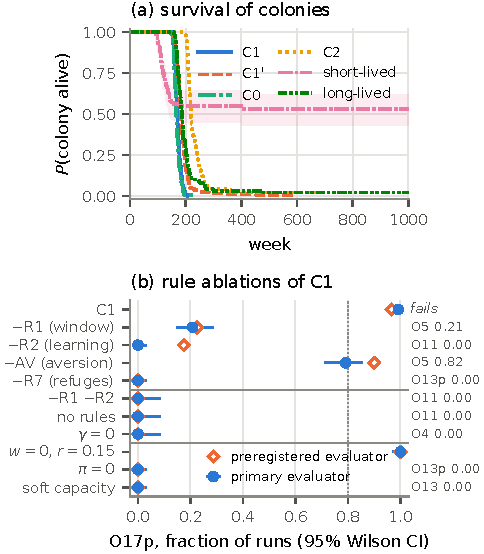
\includegraphics[width=\columnwidth]{fig_pre_rules.pdf}
  \caption{What the rules change. \textbf{(a)}~Kaplan--Meier survival of the colonies for the candidates
  ($n=200$; $T=600$, or 700 for \textsf{C2}) and the controls (the core model without the four rules and $\alpha=1.4$: short-lived,
  $a_{\max}=60$; long-lived, $a_{\max}=120$; $n=100$, $T=1000$), with log--log Greenwood bands for \textsf{C1} and
  the short-lived control. Every model with the long-lived demography dies out within a narrow window; only the
  short-lived control survives and oscillates (53 of 100 colonies alive at $T$). \textbf{(b)}~O17p of \textsf{C1}, its rule ablations
  and implementation variants with the primary evaluator (filled, 95\% Wilson interval) and the preregistered
  evaluator (open); single ablations and variants $n=120$, multiple ablations and $\gamma=0$ $n=40$. The right
  margin names the essential criterion with the lowest pass rate where O17p $<0.95$; the dotted line is the 0.8
  threshold.}
  \label{fig:res-rules}
\end{figure}

\subsection{Trajectories}
\label{sec:res-trajectories}

The time course of \textsf{C1} (Fig.~\ref{fig:res-trajectories}) is a single boom, a plateau and an extinction
by old age. The mean social state of the adults (age $\ge6$ weeks) falls below 0.5 at week 13 [13, 14], while the
population is still growing; part of this fall is dilution by pups born near $s=0$, and measured on the animals
past the plasticity window or on the founders the crossing comes at week 16, so deterioration takes of the order of
one generation, $\Gamma=t_{\rm det}/T_{\rm gen}\approx1.1$ ($t_{\rm det}\approx10$ weeks, $T_{\rm gen}\approx9$).
The socially functional growth phase is short either way (O10b in 0.02 of the runs with the adult mean, 0.28 on the
animals past the window): a phase B of 13 weeks that holds two thirds of the births, against 30 weeks in
Universe~25. The population comes within 2\% of its maximum at $t'_{\rm pk}=34$ [32, 36] weeks, 99\% of the births
have occurred by week 40, the last surviving birth is at week 59, the plateau lasts 51 [49, 53] weeks, and the
colony then ages at one week per week and dies out at week 169 [167, 171] (Kaplan--Meier median). The peak uses
$\rho_{\rm pk}=0.36$ of the damage-threshold capacity and leaves 16\% of the cells empty (Universe~25: 0.57 and
about 20\%; an agreement in sign only, since $f_0$ was used in the calibration), and 17\% of the adults form a
persistent isolated class (0.6\% in \textsf{C0}). The desirable patterns are only partly reproduced: O8 passes in
0.62 [0.56, 0.69] of the runs, O9 in 0.45 and O13b in none (SM, Table~S3). Without mortality before senescence the
maximum $t_{\rm pk}=\arg\max N$, at week 55 [50, 60], falls on the last birth before it in 69\% of the runs, 21
weeks after the plateau begins; the decline lasts $(T_{\rm ext}-t_{\rm pk})/t_{\rm pk}=2.07$ peak times with
$\arg\max N$, close to Calhoun's 1.84--2.2, but 3.97 with $t'_{\rm pk}$, so this agreement is not a robust result.
The short-lived control, the core model with the four rules switched off, $\alpha=1.4$ and a short life
($a_{\max}=60$, $a_{\rm rep}=50$ weeks), fails O11 and O13 in every run and 53\% of its colonies oscillate. \textsf{C2}, which
ties the retreat to maternal socialization, makes its isolated class a later-born cohort (O13b at least marginal in
200/200 runs against 0/200 in \textsf{C1}) but pays with its demography: O8 fails in every run, O5 falls to 0.815
and O17p to 0.705 [0.64, 0.76], against 0.98 in the \textsf{C1} ensemble of the same stage (Holm
$p=4\times10^{-14}$ over the 29 rows of the \textsf{C1}--\textsf{C2} family), whereas the calibration had predicted
no difference (SM, Table~S7).

\begin{figure*}[t]
  \centering
  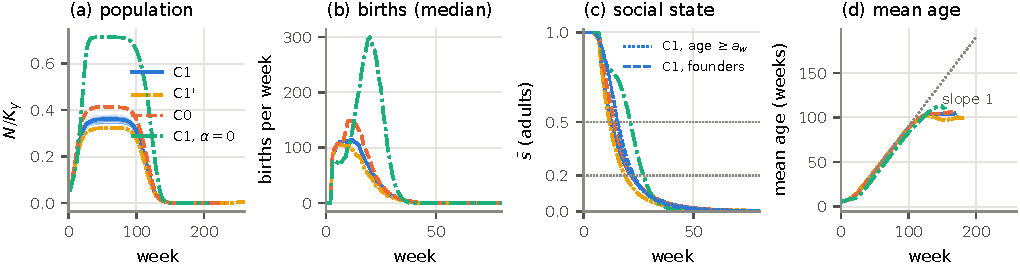
\includegraphics[width=\textwidth]{fig_pre_trajectories.pdf}
  \caption{Time course of the reference ensemble ($n=200$ each). \textbf{(a)}~Population relative to the
  damage-threshold capacity $K_\gamma=m_c|G|$: median and 10--90\% band for \textsf{C1} (thin lines are 12
  individual runs), and medians for \textsf{C1}$'$, \textsf{C0} and the $\alpha=0$ control. \textbf{(b)}~Weekly
  births (median). \textbf{(c)}~Mean social state of the adults (age $\ge6$ weeks; lines as in a), median over
  living colonies while at least half of them are alive; for \textsf{C1} also the mean over the animals past the
  plasticity window (dotted) and over the founders (dashed), which are not diluted by the newborn pups. Grey dotted
  lines: the 0.5 level of O10 and the 0.2 deterioration threshold. \textbf{(d)}~Mean age, with a reference line of
  slope one: after natality stops, the colony simply ages.}
  \label{fig:res-trajectories}
\end{figure*}

\subsection{Irreversibility: R1 and the transplants}
\label{sec:res-irreversibility}

Calhoun reports that small groups moved from mid-phase D to uncrowded universes failed to reproduce, even with
partners raised without crowding \cite{Calhoun1973,Marsden1972}. The model reproduces this (O12), but by
construction, so the transplants are a consistency check of R1 rather than a finding (Fig.~\ref{fig:res-transplant}).
Four males and four females of each \textsf{C1} colony, taken at $1.75\,t'_{\rm pk}$ (week 60; ages 37--64 weeks),
never found a colony in a \textsf{C1} enclosure (0/60), nor with healthy partners (0/120), but do in 51/60 trials
when the same animals are placed in an enclosure without R1 and R2 with individual recovery at $r=0.1$ (arm $X$;
exact McNemar $p=4\times10^{-16}$), so the preregistered prediction for arm $X$ ($\ge0.25$) holds (Q1). These
animals have $s\approx0$ (median 0.000, maximum 0.36), and fecundity scales as $s_f^2s_m$, so under R1 they cannot
found a colony with any partner. The rate in arm $X$ is a matter of age: at the preregistered sampling time
$1.75\,t_{\rm pk}$ (week 97; ages 59--80, with the fertile window closing at 80) the same colonies give 12/60, and
at week 95 in every arm, the common time that removes the confound between rule and sampling time, 5/60. A new arm
samples adults past the plasticity window with $0.2\le s\le0.5$ (median 0.36; weeks 8--11): under R1 they found a
colony in 5/60 trials, against 57/60 for the same animals in arm $X$ and 50/60 without R1, and the adult
descendants of the colonies they found settle at the social state of their parents (0.28--0.45 in \textsf{C1}).
The irreversibility of R1 + R2 is thus strict for $s\approx0$; for intermediate animals R1 acts through fecundity,
not through a collapse of the lineage, which confirms only the first part of the mean-field lineage argument of
\extended\ (SM, Sec.~S5).

\begin{figure}[t]
  \centering
  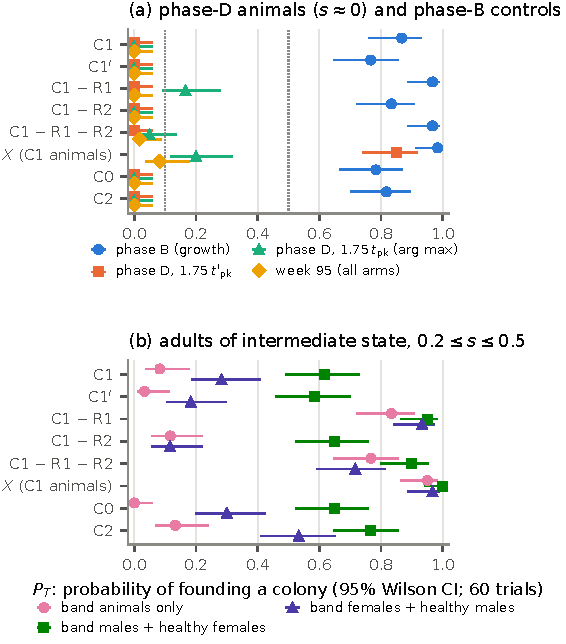
\includegraphics[width=\columnwidth]{fig_pre_transplant.pdf}
  \caption{Transplant experiments (60 replicates per arm and phase). $P_T$ is the probability that four males and
  four females moved to an empty lattice reach 80 individuals within 150 weeks. \textbf{(a)}~Animals taken in
  phase B and in phase D at three sampling times: $1.75\,t'_{\rm pk}$ of each colony, $1.75\,t_{\rm pk}$ with
  $t_{\rm pk}=\arg\max N$ (preregistered protocol), and week 95 in every arm; dotted lines mark the O12 thresholds.
  \textbf{(b)}~Adults past the plasticity window with $0.2\le s\le0.5$, alone and paired with healthy animals of
  the other sex. Arm $X$ moves the animals of the \textsf{C1} arm, the same individuals, into an enclosure without
  R1 and R2 with individual recovery at $r=0.1$.}
  \label{fig:res-transplant}
\end{figure}

\subsection{A boom of one to two generations}
\label{sec:res-boom}

Following every animal of the reference ensemble by generation shows how shallow the collapse is. The founders
deteriorate by crowding during their own adult life (they leave the plasticity window with $s=0.90$ but have
$s=0.20$ at 26 weeks of age) and produce 69\% of all births, about 6\% of their potential fecundity. Their
offspring are born at $s_{\rm nb}=w\,s_f\simeq0.19$, below the deterioration threshold, and gain only $+0.04$ by
the end of the window, because their teachers are already deteriorated. The net reproductive number falls by a
factor of about ten in a single step, from 3.8 daughters per founder female to 0.40 in the first generation born,
then to 0.11 and 0.05; the second generation adds 27.6\% of the births and the third and later ones 3.2\%. The
mean generation of the births is 1.34 in \textsf{C1}, against 1.95 [1.90, 1.99] in the long-lived control and 1.59
in \textsf{C1} without its rules, whose first generation still has $R_{\rm net}=1.21$ and 0.66: the rules, R2 in
particular, shorten the generational depth, because pups no longer inherit the competence of the few healthy
mothers. R2 does not produce a cascade over many generations; it makes the failure of the first generations born
during the boom irreversible for the colony, in every variant of Sec.~\ref{sec:res-robustness}. Births are
front-loaded: half of them occur before $0.36\,t'_{\rm pk}$ and 93\% before $0.8\,t'_{\rm pk}$, the start of the
window of the strict O13b criterion, which therefore cannot pass. In \textsf{C1} the isolated and the crowded
classes are born together (median birth weeks 10 and 11), so the persistent isolated class is made of refugees of
the early boom, most of whom entered the refuges as pups, not of Calhoun's late-born ``beautiful ones'';
\textsf{C2} obtains the later-born class (median birth week 22 against 11) at the demographic cost described
above. The simulated dynamics is a boom of one or two generations rather than Calhoun's multi-generational
sequence (Sec.~\ref{sec:discussion}).

\subsection{Robustness and the central limitation}
\label{sec:res-robustness}

Fig.~\ref{fig:res-rob} reports \textsf{C1} and \textsf{C1}$'$ under the robustness variants ($n=200$ each); by the rule fixed before the runs, a variant preserves the result if O17p $\ge0.8$ (SM,
Table~S9). With a constant background hazard $\mu_{\rm bg}$ at all ages the plateau shrinks (51 weeks at 0, 35 at
0.001, 17 at 0.003 and 10 at 0.008 per week) and O17p falls to 0.83, 0.63, 0.55 [0.48, 0.62] and 0.06 in
\textsf{C1} (0.67, 0.38, 0.28 and 0.04 in \textsf{C1}$'$). The only criterion that fails is O5, and it fails
through its timing clause, not through its level: at $\mu_{\rm bg}=0.003$ O5 is MARGINAL in 83 of the 200 runs
and FAIL in 7, because the start of the plateau moves from week 34 to 29 while $t_{B99}$ moves from 40 to 43, so
$(t_{B99}-t'_{\rm pk})/t'_{\rm pk}$ crosses the 0.5 threshold of O5 while natality still ends with the population
near its maximum. The classes, O11 and the low peak are unchanged, and O17p restricted to the criteria that
discriminate against the null models (O11 at six weeks, O13, O13p and the anti-patterns) is 1.00 at every
$\mu_{\rm bg}$. With initial ages drawn uniformly from 4--52 weeks instead of all equal, O17p is 0.93 [0.89, 0.96];
from 4--80 weeks, which includes post-reproductive founders, 0.63 [0.56, 0.69] (0.68 and 0.31 in \textsf{C1}$'$),
again through the timing clause of O5 (73 MARGINAL and 1 FAIL of 200) and with the restricted outcome at 1.00. The
timing of the end of natality relative to the start of the plateau is therefore a property of the synchronous
initial condition and of the absence of mortality before senescence, not of the rules; the end of natality near
the maximum itself persists. Since O5 is generic, these variants remove the generic part of the primary outcome,
not the part that carries evidence for the rules; but the primary outcome \emph{as defined} holds only without,
or with very weak, background mortality, which is the central limitation of the result
(Sec.~\ref{sec:discussion}). The other variants preserve it: a nest period of three weeks gives 0.835 [0.78, 0.88],
borderline because the interval contains 0.8 (0.60 in \textsf{C1}$'$); a random sequential update gives 1.00 with
the hard and 0.995 with the soft refuge capacity; and the exact refuge capacity gives 0.995 against 0.995 with a
single-pass admission. Pups born above the deterioration threshold ($s_{\rm base}=0.25$ or 0.5) give O17p
of 0.08 and 0.00, entirely through O11 scored at six weeks; scored at the age $a_w$ the same runs give O17p of
0.965 and 0.76, because by the end of the window the late cohorts are below 0.2 whatever their birth state. Over
lattice sides $L=15$--60 at fixed density $N_0/L^2=0.44$ ($n=60$; SM, Table~S10), the peak density (0.35--0.37)
and the persistent fraction (0.17--0.18) do not change and O17p rises from 0.82 [0.70, 0.89] at $L=15$ to 1.00 at
$L\ge45$; the spread of the extinction time falls from 0.15 to 0.08 together with the relative spread of the last
birth (0.58 to 0.18), while $T_{\rm ext}-t_{\rm last}$ stays at 110--112 weeks [Fig.~\ref{fig:res-rob}(c)]: the
spread of $T_{\rm ext}$ is that of the end of natality, and a narrow spread is not a signature of the rules (0.045
without attraction, 0.160 in the long-lived control). O17p reaches 0.8 only for seeding densities
$0.2\lesssim N_0/L^2\lesssim0.9$, and with Calhoun's four founding pairs no run is Calhoun-like (the best point of
an exploratory founder plane reproduces O1--O3 together with O17p in 0.43 [0.27, 0.61] of the runs). Around
\textsf{C1} the primary outcome holds over part of the explored planes (30 runs
per cell): O17p is at least 0.83 for $w\le0.3$ and $r\le0.10$ and falls at $w\ge0.5$ and $r\ge0.2$ through O11;
every finite window $a_w\le24$ gives certain extinction; in the $(\alpha,\kappa)$ plane O17p is at least 0.8 at 34
of the 48 points with $\alpha\ge2$, failing where the free space of O4 is lost; and a persistent isolated class
requires a strong refuge preference and a total refuge capacity $f_Rc_R\ge0.4$.

\begin{figure*}[t]
  \centering
  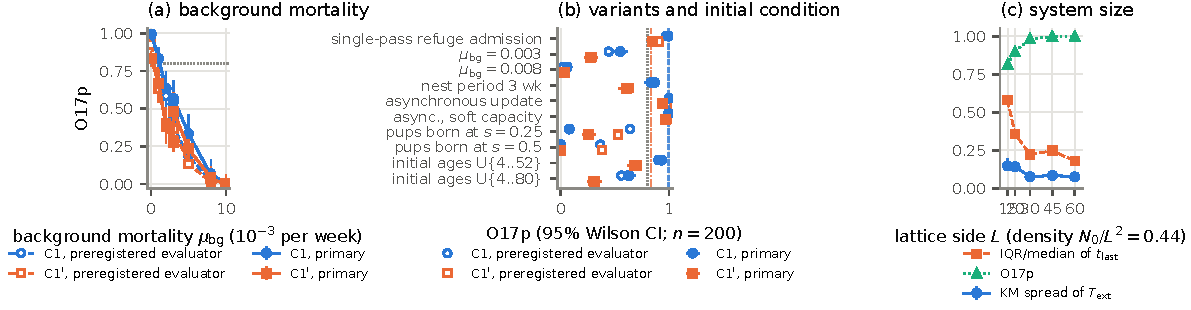
\includegraphics[width=\textwidth]{fig_pre_robustness.pdf}
  \caption{Robustness of the primary outcome ($n=200$ per arm unless stated). \textbf{(a)}~O17p against the
  background mortality $\mu_{\rm bg}$ for \textsf{C1} and \textsf{C1}$'$ ($n=60$ at the intermediate values), with
  the primary (filled) and the preregistered evaluator (open); dotted line: the 0.8 threshold. \textbf{(b)}~Variants
  of \textsf{C1} and \textsf{C1}$'$ (vertical lines: the reference ensembles and the 0.8 threshold).
  \textbf{(c)}~Lattice side at fixed seeding density ($n=60$ per size): Kaplan--Meier spread of the extinction
  time (interquartile range over median), relative spread of the last birth, and O17p.}
  \label{fig:res-rob}
\end{figure*}

\subsection{Feasible region and sensitivity}
\label{sec:res-global}

Over two independent 15-factor Latin hypercubes (400 points, 10 runs each, plus 40 runs at 18 boundary points),
2.0\% [0.7, 3.6] of the points are Calhoun-like with the primary evaluator ($k/n\ge0.8$; bootstrap over points),
the mean of O17p over the box is 4.0\% [2.6, 5.9], and an empirical-Bayes fraction that shrinks each point towards
a logistic emulator is 1.8\% [0.7, 3.2]; with the preregistered evaluator the same runs give 7.2\%, 11.0\% and 6.9\%
[4.8, 9.2]. Every such fraction is relative to the box and to the sampling scales of Table~\ref{tab:params}. Part of
the small fraction is definitional and part is mechanism: with $c_R=3$ refuge residents exceed the isolation
threshold and none of the 100 such points is Calhoun-like; restricting successively to $c_R\le2$, $m_c\le10$,
$f_Rc_R\ge0.3$ and $\pi\ge100$ (chosen after the runs) raises the fraction to 2.7\%, 3.1\%, 5.6\% and 10.8\%
[2.7, 21.6], and even then 33 of the 37 points fail, through O11 (16), the persistence of the class (14), O5 (9)
and O4 (9). The Sobol' decomposition (11 factors; SM, Fig.~S1) finds O17p equal to zero at 78\% of its points; its
total indices are led by $c_R$ ($0.49\pm0.16$), $w$ (0.43), $\kappa$ (0.41), $r$ (0.32) and $m_c$ (0.31), which
cannot be ordered, and its first-order indices add up to only 0.15, so it is almost entirely interactions, while
the continuous outputs are nearly additive; the window $a_w$ does not exceed its noise floor.

\subsection{Confirmatory tests}
\label{sec:res-Q}

With the primary evaluator six of the seven preregistered null hypotheses are rejected after Holm adjustment and
the quantitative predictions are met for Q1, Q3, Q4 and Q7 and not for Q2, Q5 and Q6; with the preregistered
evaluator five are rejected and four predictions hold (Q3, Q4, Q6 and Q7). The two counts differ in three places:
Q2 is rejected only with the primary O5, the prediction of Q1 holds only at the earlier transplant time, and the
prediction of Q6 holds only with the preregistered O11 (SM, Table~S7). Of the predictions that hold, Q1 is a
consistency check of R1 and Q4 of the demography: once births stop, extinction is the death of the last survivor
of a closed, ageing population, so the expected $T_{\rm ext}-t_{\rm last}$ grows one-to-one with $a_{\max}$ and
only logarithmically with the size of the last cohort (slope $0.996\pm0.014$ over 300 runs). Q3 confirms a
near-deterministic collapse against the short-lived control (200/200 extinct by $T=600$ against 47/100 by $T=1000$; coefficient
of variation of $T_{\rm ext}$ 0.066 [0.059, 0.071]), but the long-lived demography alone goes extinct in 0.98--1.00
of the runs ($p=0.11$), so extinction does not discriminate. Q5, a coexistence band of O13 centred at the
preferred occupancy $n^*=1/\kappa-1/\alpha\approx m_c$, is refuted in the opposite direction (O13 passes in at
least 95\% of the runs at 46 of the 49 points with $n^*>0.5$): with refuges the isolated class no longer depends on
the balance between attraction and aversion. Q6, that the window weighs less than the learning rate ($0<\theta<1$
in $\log r+\theta\log a_w$), is not supported with the primary evaluator: the Calhoun-like boundary of the
$(r,a_w)$ plane is nearly vertical in $r$ and the single-index fit gives $\hat\theta=-0.15$ [$-0.20$, $-0.05$] in a
model that an additive one beats ($\Delta{\rm QAIC}=28$); with the preregistered evaluator it gives $\hat\theta=0.30$
[0.15, 0.50]. Q7 confirms an endogenous collapse without crowding damage: at $\gamma=0$ the four subcritical points
($w\le0.1$, $r\le0.03$) went extinct in 120/120 runs while all 30 \textsf{C1} colonies exploded, but the colonies
of the corner first overshoot the capacity ($\rho_{\rm pk}=0.91$--1.60), so none is Calhoun-like; with the window
varied, the transition in $\Lambda=r\,a_w$ falls in the same grid bracket for $a_w=12$ and 24 and one step lower
for $a_w=6$, and the preregistered logistic model is separated (51 of 54 points have $P_{\rm ext}\in\{0,1\}$), so no
single exponent is reported as inference (SM, Sec.~S4). The mean-field analysis of \extended\ mostly describes the
short-lived control (a superstable limit cycle sustained by healthy pockets of uncrowded individuals, without
secular drift of the peaks); what carries over to \textsf{C1} is the phase-D law of Q4, the capacity bound of the
persistent class $\Phi^{\rm pers}_{\rm BO}\le f_Rc_R|G|/N_{\rm pk}$, and the heuristics behind Q6 and Q7, which the
data support only in part.

\section{Discussion}
\label{sec:discussion}

\paragraph*{The envelope is generic; the rules add the classes.}
The main lesson of the production runs is a negative one. A long-lived demography alone, without any of the new
rules, drives 199 of 200 colonies to extinction: once natality stops, the colony simply ages out. Neither extinction
nor the rest of the envelope is a result of the rules. With crowding damage and the calibrated attraction, the
candidate without its four rules has a low peak with free space (the primary O4 passes in 200 of 200 runs, with a
peak at 0.45 of the damage-threshold capacity and 74\% of the cells empty), an end of natality and no rebound;
scored at the end of the plasticity window, its late-born cohorts also fail to acquire social competence (O11 in
0.755 of the runs, and 0.81 in the long-lived control), through accumulated crowding damage. Of the eight essential
criteria, five (O4, O5, O6, O7 and O10) pass in at least two of the four null models and carry no evidence for the
rules. What the rules add is the coexistence of crowded and isolated deteriorated classes (O13). It is absent in the
long-lived control, without crowding damage and without the rules, and present with refuges alone (1.00 in
\textsf{C1}$'$) or crowd aversion alone (0.92); full inheritance without social learning also produces it. Other
patterns hold by construction and only verify the implementation: the isolated class is persistent (O13p) because
the refuge capacity equals the isolation threshold, and transplanted late-phase animals never found a colony (O12)
because under R1 an adult cannot recover and conception scales with the social state of both partners. The
non-trivial part is upstream: the colony drives essentially every adult to $s\approx0$, and crowding damage alone
largely achieves it.

\paragraph*{A boom of one or two generations.}
The founders deteriorate by crowding during their own adult life; their offspring, about 70\% of all births, are
born below the deterioration threshold and learn from adults who have already deteriorated. The net reproductive
number falls from 3.8 in the founders to 0.40 in their daughters, so natality stops within about one generation.
The null models have a \emph{deeper} boom (mean generation of the births 1.59 without the four rules, 1.34 in
\textsf{C1}): the rules, R2 in particular, shorten the generational depth rather than create a long cascade. The
phases appear in Calhoun's order, but B and C are compressed and an artificial plateau precedes D. The ratio of the
deterioration time to the generation time, $\Gamma\approx1.1$ against about 3.5 in Universe~25 with a different
operational definition, is a heuristic comparison of time scales, not the cause of the shallow boom. Within this
transient, crowding damage is the trigger, social learning the amplifier, the plasticity window the ratchet, and the
refuges make the isolated class persistent; without R1 the refuges become pockets of low density where deteriorated
animals recover and breed again (the primary outcome falls to 0.21).

\paragraph*{The central limitation: demography and initial condition.}
The model has no mortality before senescence, and its initial condition is a synchronous cohort of 400 healthy
four-week-old animals. With a background hazard of 0.003 per week at all ages the primary outcome falls from 0.995
to 0.55 (0.06 at 0.008 per week), and with initial ages spread over 4--52 or 4--80 weeks it is 0.93 and 0.63. In
every case the only criterion that fails is O5, by its timing clause. Natality still ends with the population near
its maximum, but the deaths bring the start of the plateau forward (from 34 to 29 weeks at 0.003 per week) while the
end of natality hardly moves (40 to 43 weeks), so O5 becomes marginal, as in 83 of the 90 failing runs at 0.003 per
week and 73 of the 74 with ages over 4--80 weeks. O13, O13p and O11 pass in every run of these arms. The dependence
is thus on the timing of the end of natality relative to the start of the plateau, a generic criterion that
discriminates against no null model and rests on a post hoc choice of that start. It is neither evidence against
what the rules add nor for it, but the primary outcome of 0.995 overstates how robustly the full conjunction of
patterns is reproduced.

\paragraph*{Circularity, scope and minimality.}
The same patterns were used to \emph{choose} the rules and to \emph{report} them, with no pattern held out, so their
fulfilment shows that they are \emph{possible} under local rules, not that they were predicted. Global robustness
is limited and relative to the sampled box: over two 15-factor Latin hypercubes the mean primary outcome is 0.040
[0.026, 0.059], and 2.0\% of the points are Calhoun-like. With at most one lattice step per week the animals are
almost sessile on the scale of the deterioration, unlike Calhoun's mice, and the coexistence of classes is lost with
more movement sub-steps. Minimality is conditional on the thresholds: the minimal set R1, R2 and R7 (\textsf{C1}$'$)
gives the primary outcome in 0.835 [0.78, 0.88] of 200 runs, borderline, and in 0.33 with a class threshold of 15\%
instead of 10\%; crowd aversion contributes but is not necessary in the preregistered sense.

\paragraph*{What is not reproduced.}
From four founding pairs a colony spreads as a slow front, and no point of an exploratory founder plane is
Calhoun-like (primary outcome at most 0.37). The persistent isolated class is made of refugees of the early boom,
most of whom entered the refuges as pups, not of a late-born cohort like Calhoun's beautiful ones. Total infant
mortality and the female bias of the remnant are not reproduced, because conception and pup survival decline
together and there is no sex-specific mortality. The model of Gwizdałła and Duś \cite{GwizdallaDus2026} reproduces
the founder phase and the timing of the curve, which ours does not, with a daily step, fitted life tables and
deviation factors triggered by the total population. Ours shows that local rules, without population-level
switches, produce coexisting classes of deteriorated animals, one of them persistent, on top of an envelope that
crowding damage and the demography already give. Both agree that replicate variability is large and that Calhoun's
trajectory is one admissible outcome among many. Making the required patterns and their thresholds explicit and
testable run by run against null models is, in our view, the main methodological contribution of this work;
background mortality, gestation, a founder protocol with realistic mobility and held-out patterns are the natural
next steps. We make no claim about human populations.


\section*{Data availability}
All code, simulation outputs and analysis scripts are available in the repository \repourl; the version
used in this paper (release v1.0) is archived in Zenodo, \zenododoi{10.5281/zenodo.23111283}. The model is implemented in the Python package
\texttt{u25}, and the candidates of this paper are the presets \texttt{calhoun\_C1p} (\textsf{C1}$'$) and
\texttt{calhoun\_C1} (\textsf{C1}). The numbers quoted here are taken from the extended version, whose results are
dumped, with their ensembles, to \texttt{results\_v2/results\_numbers.json}, and all figures are regenerated from the scripts of the
repository, as described in its README. An extended version with all analyses (the calibration, the mean-field analysis and the complete
results), the full ODD description, the code and the data is available in the repository \repourl.

\section*{Declaration of generative AI use}
The author designed the project and provided a preliminary implementation of the agent-based model, together with a
draft describing its objectives and interaction rules, which were taken as the starting point. Claude (Anthropic),
used through Claude Code in a multi-agent setting (agents with the roles of mathematician, physicist, programmer and
literature reviewer, coordinated by a principal agent), contributed to the reimplementation and extension of the
code, the simulations, the statistical analysis, the literature review and the writing of the manuscript. An
independent system of Claude agents carried out an internal review in three rounds. The author supervised the work,
reviewed all of its content and takes full responsibility for it.

\bibliographystyle{apsrev4-2}
\bibliography{refs}

\end{document}
